\frame
{
\frametitle{Gráficos}
\framesubtitle{Tests}
\begin{center}
	Total de instancias: 30
\end{center}
\begin{itemize}
	\item 10 instancias con 200 variables
	\item 10 instancias con 300 variables
	\item 10 instancias con 400 variables
\end{itemize}
\begin{block}{SA}
\begin{itemize}
	\item 50 ejecuciones por cada instancia.
\end{itemize}
\end{block}
\begin{block}{AE + SA}
\begin{itemize}
	\item 100 ejecuciones por cada instancia.
\end{itemize}
\end{block}
}

\frame
{
\frametitle{Gráficos}
\framesubtitle{Mínimo de restricciones insatisfechas}
\begin{center}
	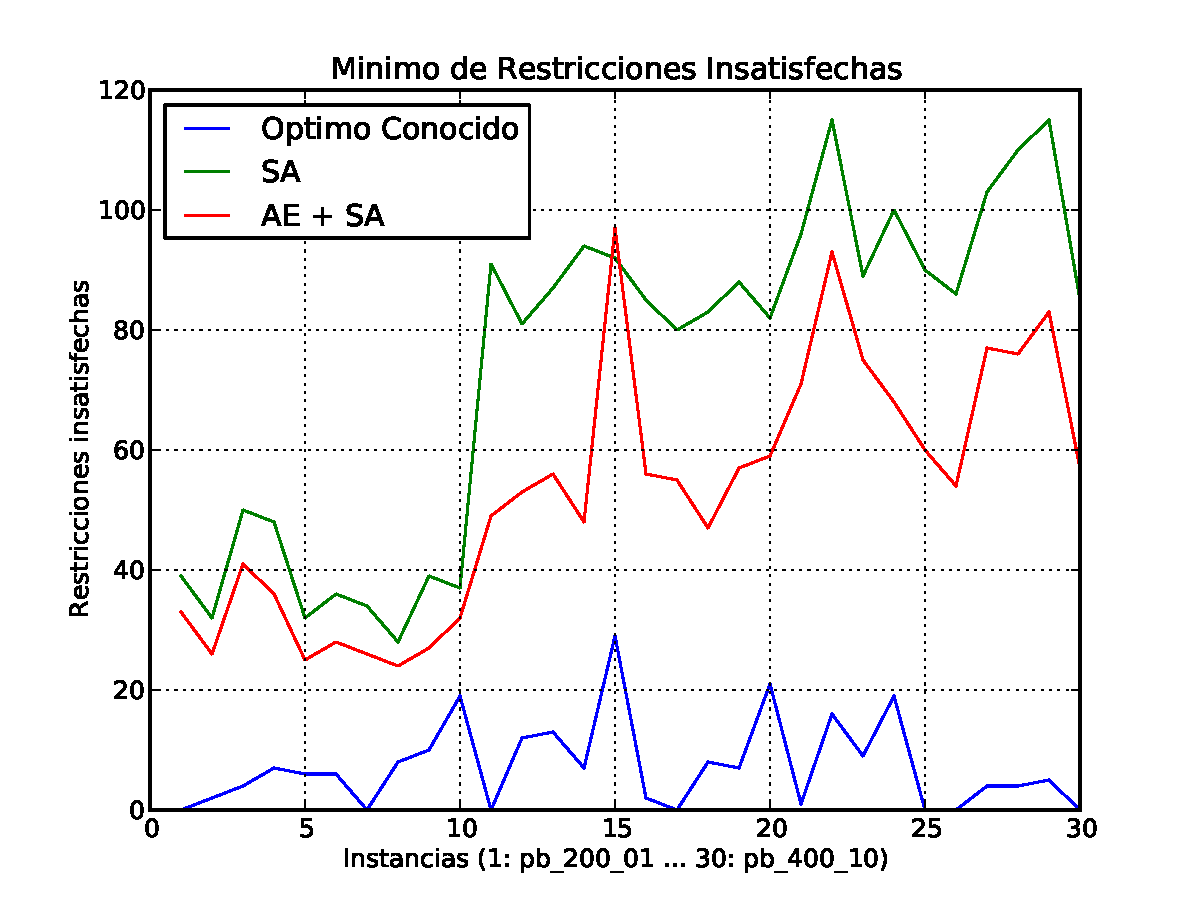
\includegraphics[width=0.8\textwidth]{img/min}
\end{center}
}
\frame
{
\frametitle{Gráficos}
\framesubtitle{Máximo de restricciones insatisfechas}
\begin{center}
	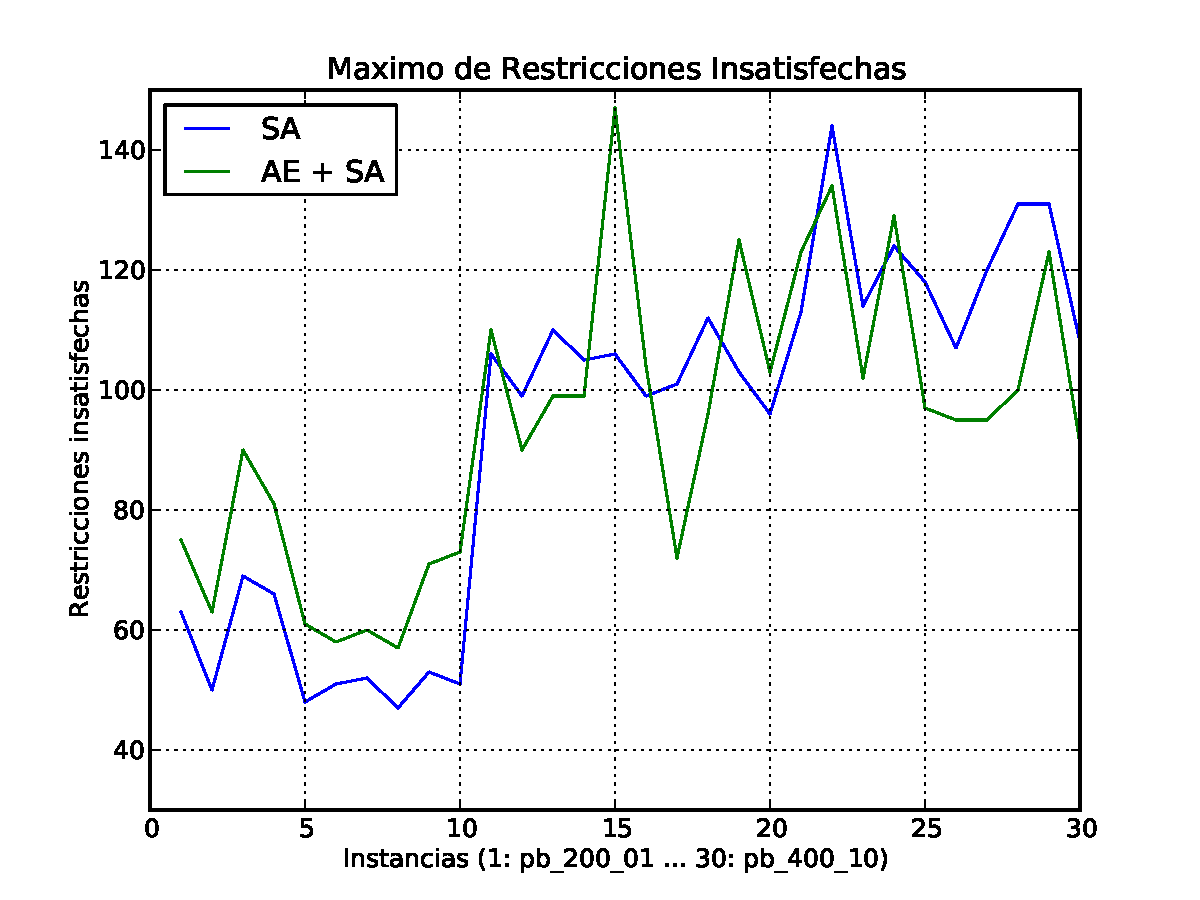
\includegraphics[width=0.8\textwidth]{img/max}
\end{center}
}
\frame
{
\frametitle{Gráficos}
\framesubtitle{Promedio de restricciones insatisfechas}
\begin{center}
	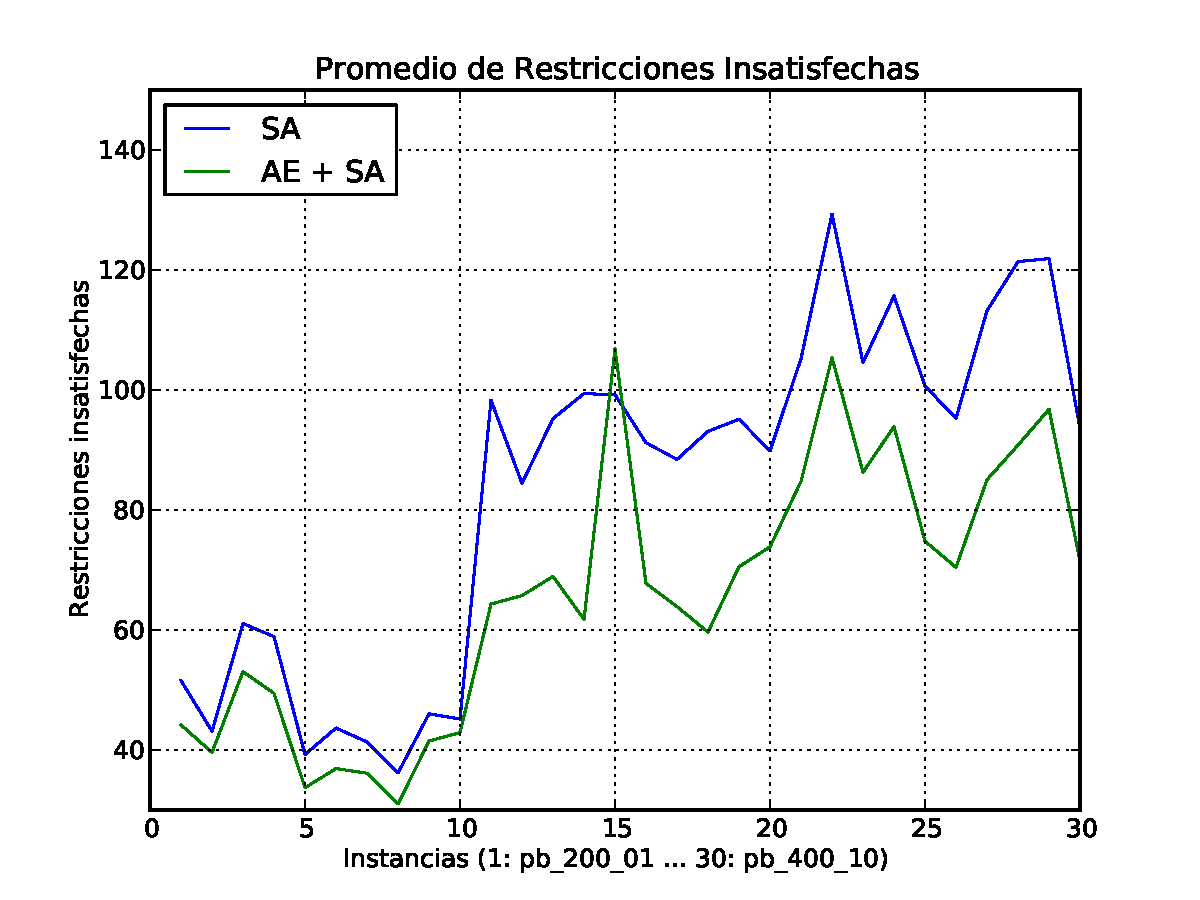
\includegraphics[width=0.8\textwidth]{img/prom}
\end{center}
}
\frame
{
\frametitle{Gráficos}
\framesubtitle{Desviación estándar de restricciones insatisfechas}
\begin{center}
	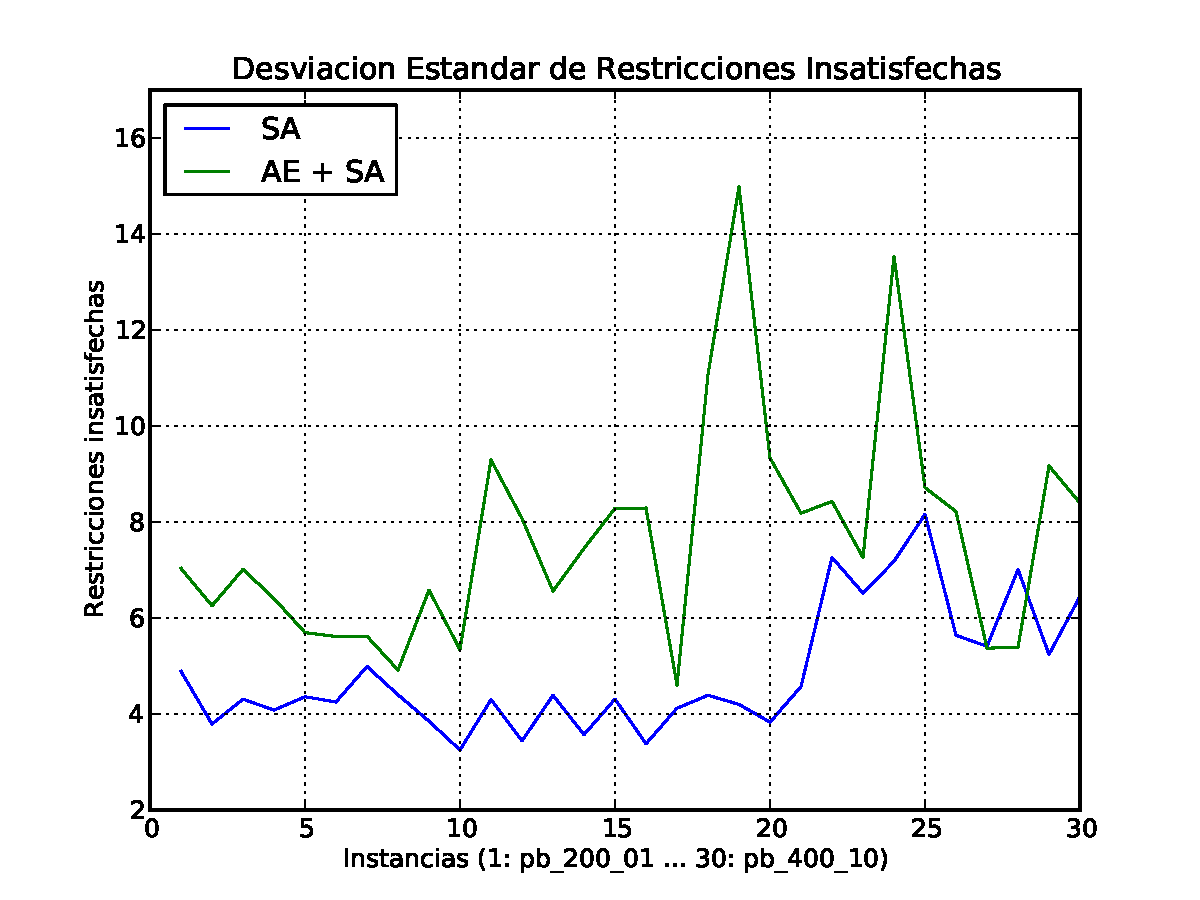
\includegraphics[width=0.8\textwidth]{img/s}
\end{center}
}
\frame
{
\frametitle{Gráficos}
\framesubtitle{Promedio tiempo de ejecución}
\begin{center}
	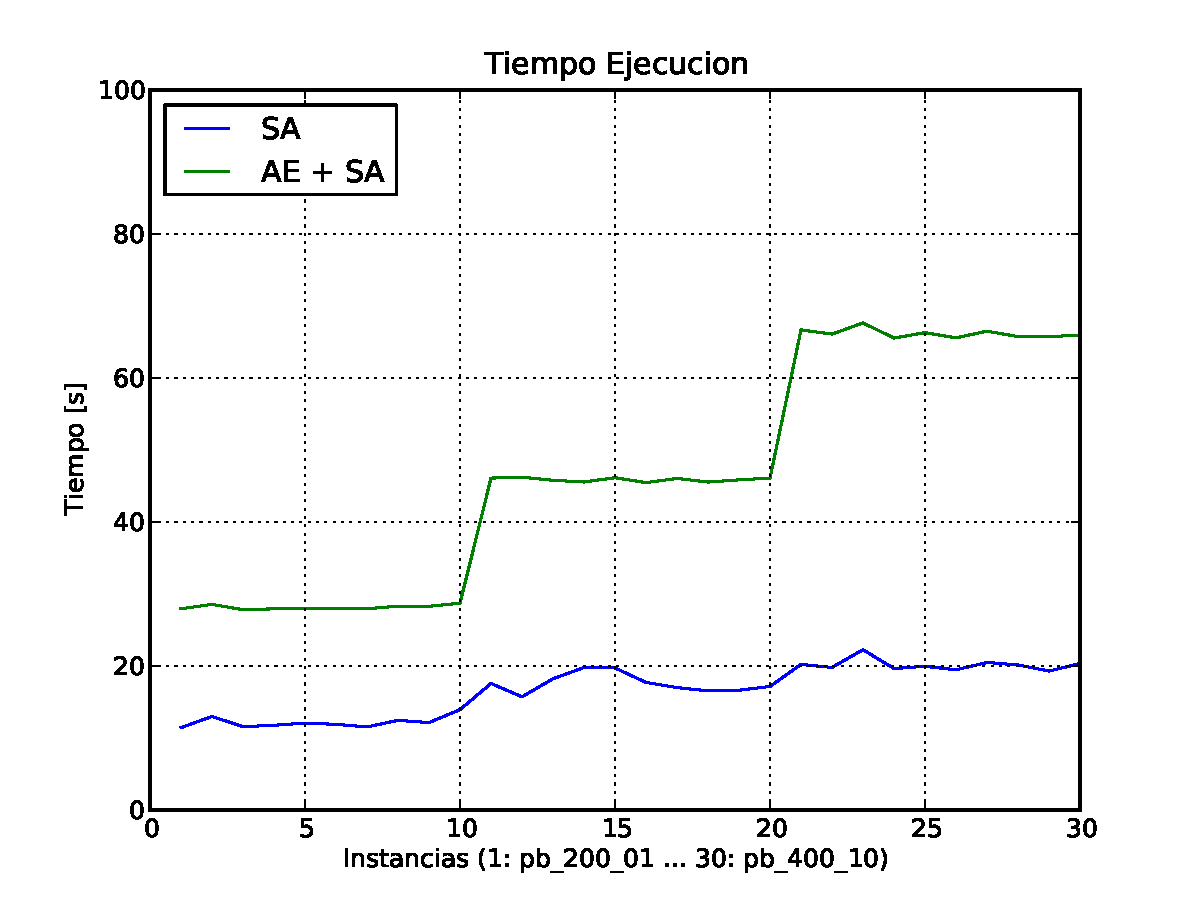
\includegraphics[width=0.8\textwidth]{img/tiempo}
\end{center}
}
